\documentclass[10pt, titlepage, oneside, a4paper]{article}
\usepackage[T1]{fontenc}
\usepackage[english]{babel}
\usepackage{ifpdf}
\usepackage{amssymb, graphicx, fancyheadings}
\usepackage{rotating}
\usepackage{nomencl}
\makeglossary
%\usepackage{hyperref}

\addtolength{\textheight}{20mm}
\addtolength{\voffset}{-5mm}
\renewcommand{\sectionmark}[1]{\markleft{#1}}

\def\inst{Computing Science}
\def\typeofdoc{Final Report}
\def\course{Software Engineering, Spring 2010, 15 hp}
\def\pretitle{Project 3}
\def\title{The Greed Game}
\def\namea{Fredrik Dahlberg}
\def\nameb{Marcus Karlsson}
\def\namec{Emil Eriksson}
\def\usernamea{c07fdg}
\def\usernameb{marcusk}
\def\usernamec{c07een}
\def\emaila{\usernamea{}@cs.umu.se}
\def\emailb{\usernameb{}@cs.umu.se}
\def\emailc{\usernamec{}@cs.umu.se}
\def\path{edu/pvt/lab3}
\def\graders{Tor Sterner Johansson}

\def\fullpatha{\raisebox{1pt}{$\scriptstyle \sim$}\usernamea/\path}
\def\fullpathb{\raisebox{1pt}{$\scriptstyle \sim$}\usernameb/\path}
\def\fullpathc{\raisebox{1pt}{$\scriptstyle \sim$}\usernamec/\path}

\begin{document}

	\begin{titlepage}
		\thispagestyle{empty}
		\begin{large}
			\begin{tabular}{@{}p{\textwidth}@{}}
				\textbf{Ume� University \hfill \today} \\
				\textbf{Department of \inst \hfill } \\
				\textbf{\typeofdoc} \\
			\end{tabular}
		\end{large}
		\vspace{10mm}
		\begin{center}
			\LARGE{\pretitle} \\
			\huge{\textbf{\course}}\\
			\vspace{10mm}
			\LARGE{\title} \\
			\vspace{5mm}
			\begin{large}
				\begin{tabular}{ll}
					\textbf{Name} & \namea \\
					\textbf{Email} & \texttt{\emaila} \\
					\\
					\textbf{Name} & \nameb \\
					\textbf{Email} & \texttt{\emailb} \\
					\\
					\textbf{Name} & \namec \\
					\textbf{Email} & \texttt{\emailc} \\
				\end{tabular}
			\end{large}
			\vfill
			\large{\textbf{Grader}}\\
			\mbox{\large{\graders}}
		\end{center}
	\end{titlepage}

	\lfoot{\footnotesize{\usernamea, \usernameb, \usernamec}}
	\rfoot{\footnotesize{\today}}
	\lhead{\sc\footnotesize\title}
	\rhead{\nouppercase{\sc\footnotesize\leftmark}}
	\pagestyle{fancy}
	\renewcommand{\headrulewidth}{0.2pt}
	\renewcommand{\footrulewidth}{0.2pt}

	\pagenumbering{roman}
	\tableofcontents
	
	\newpage

	\pagenumbering{arabic}
	
	\section{Description}
	
	The project aims to implement a dice game called Greed. It is a turn-based game where a player throws a number of dice and has the ability to receive scores depending on a set of rules.

	A player has to reach a lower limit called the bust limit. If the first roll in a turn does not reach that limit the player is bust and the turn will be given to the next player. If the player does not go bust it will have the option to either stop and register the collected scores or roll again and try to collect more points. There must always be at least one die that scores in each roll. If no die scores the player goes bust and the score collected in that turn will be lost. When a die has scored it cannot be used again until all dice has scored.

	This project will implement a GUI-based version of the Greed game. Any number of players may enter or leave the game at any time and they should be able to play from different computers.

	Computer controlled players should also be supported. At least the following four types should be implemented.

	\begin{itemize}
	\item \emph{Coward}, will play safe and not take any risks.
	\item \emph{Random}, will play randomly.
	\item \emph{Clever}, will play cleverly and make tactical decisions, i.e. based on the scores of the other players.
	\item \emph{Gambler}, will play to win as fast as possible by taking very high risks.
	\end{itemize}
	
	These players will be discussed more in depth in Section \ref{sec:design}.
	
	\section{Design}
	\label{sec:design}
	
	The design is finished and the only remaining unit subject to large changes is the user interface which might not change a lot visually during the implementation but quite a lot under the hood.
	
		\subsection{User Interface}
		
		%\begin{figure}[h!]
		%	\centering
		%		\ifpdf
		%			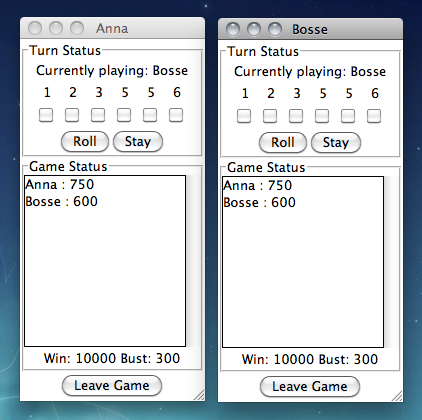
\includegraphics[width=0.7\textwidth]{prototype4.png}
		%		\fi
		%	\caption{A view of the graphical user interface}
		%	\label{fig:gui}
		%\end{figure}
	
		The user interface (seen in \figurename{} \ref{fig:gui} on \pagename{} \pageref{fig:gui}) is implemented in Ruby/Tk.
		
		The concept is that each player will have their own window from where they can follow the game and respond when it is their turn. The window has two major components. An upper frame where information is presented about the current turn like the name of the current player and the dice throws. This is also were the player can decide to roll or stop and register collected points. If the player wants to roll again he or she can select one or more dice to save using the checkboxes. 
		
		The lower frame contains overall information about the current game. This includes a list of scores, the limit for winning as well as the limit required for not being bust. The player can leave the game by pushing the button lowest down in the window.
		
		\subsection{Software}
		\begin{figure}[t]
			\centering
				\ifpdf
					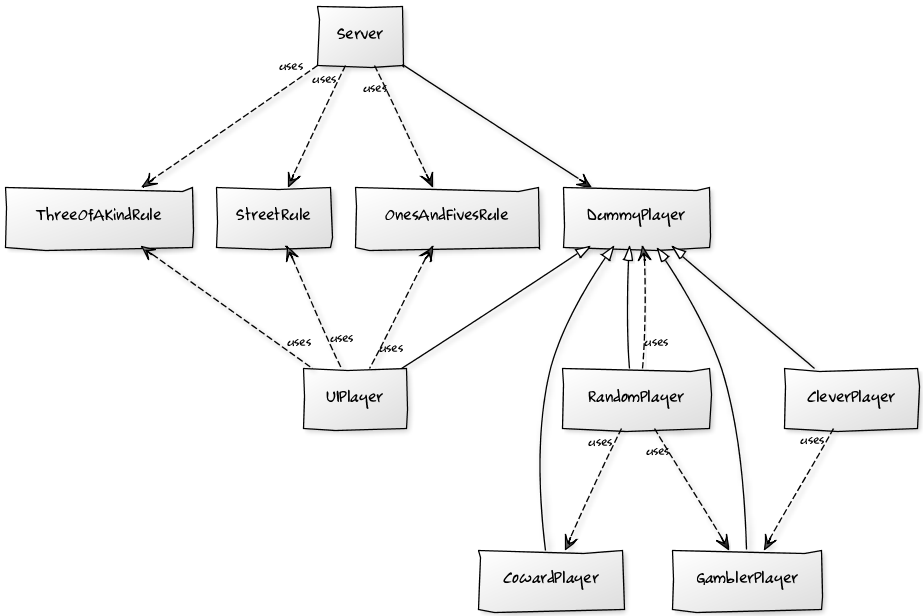
\includegraphics[angle=90,width=\textwidth]{uml.png}
				\else
					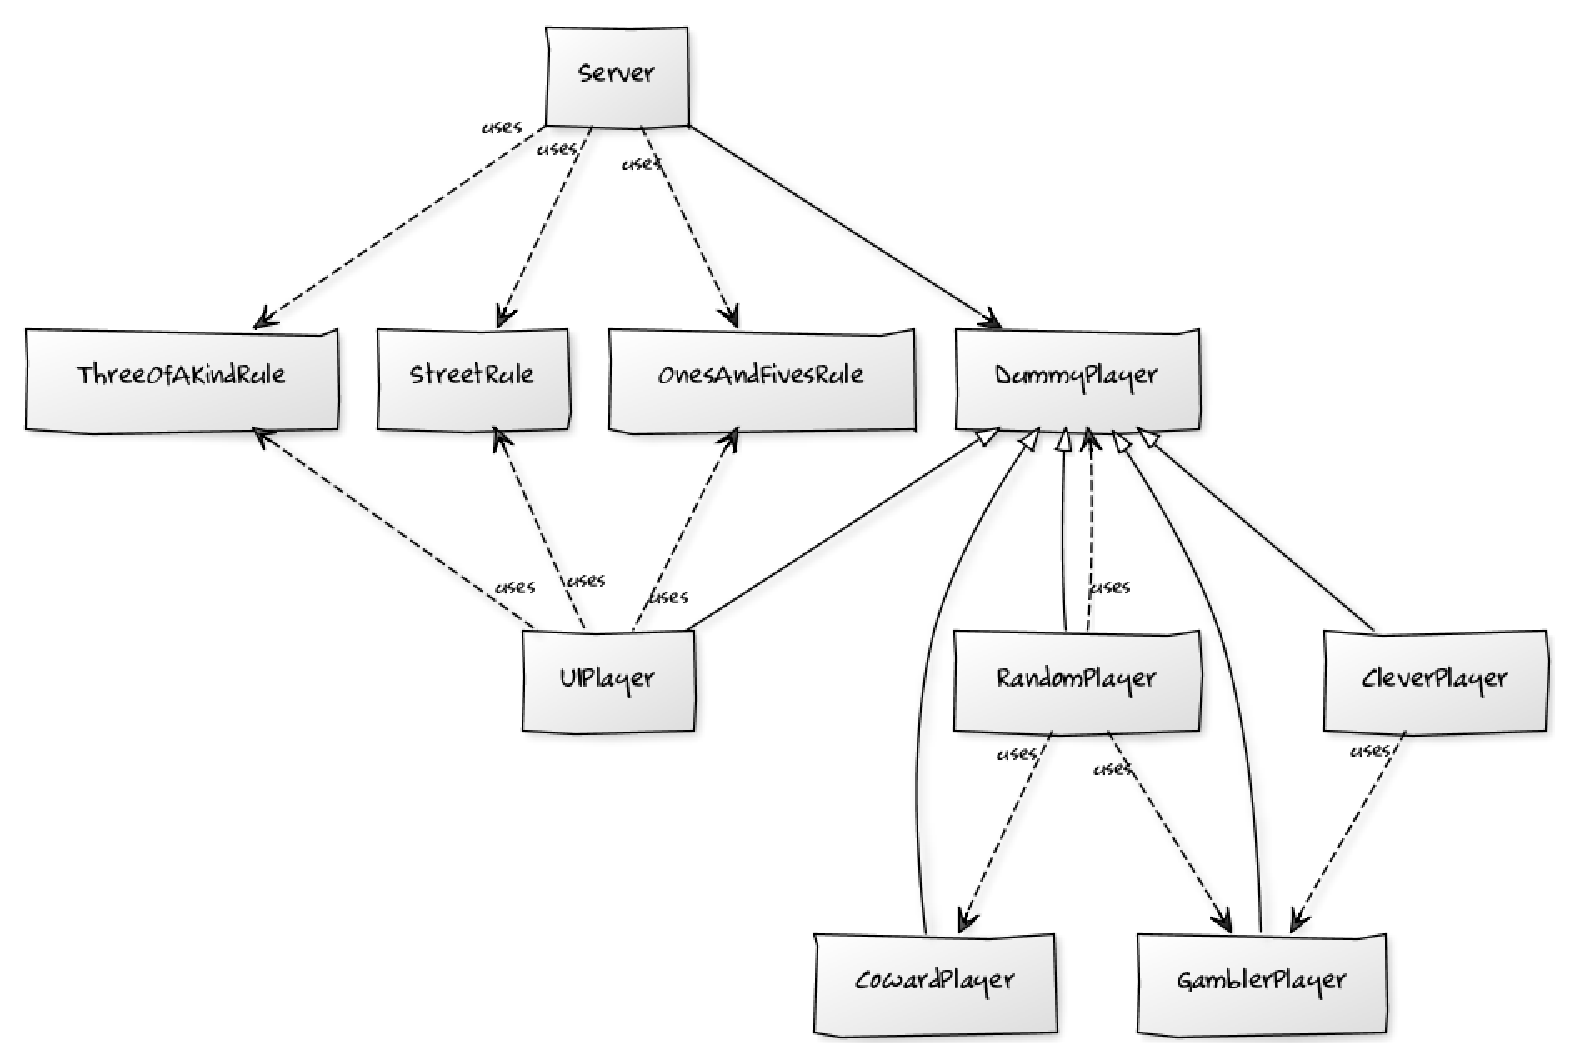
\includegraphics[angle=90,width=\textwidth]{uml.eps}
				\fi
			\caption{Class diagram over the software}
			\label{fig:uml}
		\end{figure}

		The software uses a structure similar to the client/server paradigm. A class diagram of the software can be seen in \figurename{} \ref{fig:uml} on \pagename{} \pageref{fig:uml}.
		\begin{itemize}
			\item A {\tt Server} which, with the help of dRuby\footnote{dRuby is a part of ruby which works similar to JavaRMI. It allows for invocation of methods on objects which might ''live'' in other processes on other hosts.}, communicates with local and remote clients.
			\item Several different players which implements more or less intelligent computer players and acts as remote clients when they are created in a different process than the server.
				\begin{itemize}
					\item {\tt DummyPlayer} a really dumb player which always rethrows all dice.
					\item {\tt CowardPlayer} always saves the score.
					\item {\tt GamblerPlayer} tries to maximize the score for each round taking large risks.
					\item {\tt RandomPlayer} randomly asks another implementation what it should do. Currently uses {\tt DummyPlayer}, {\tt CowardPlayer} and {\tt GamblerPlayer}.
					\item {\tt CleverPlayer} adapts playing style according to where it is on the scoreboard. If it's in the lead it plays very safe and when another player is in the lead it takes higher risks in order to get more points.
				\end{itemize}
			\item A \emph{special} player (called {\tt UIPlayer} in \figurename{} \ref{fig:uml}) which displays a user interface and lets the user interact with the game. This player can also communicate with a remote server.
		\end{itemize}
		
		The server (and the UI) uses several dynamically loaded rules to determine the score for each throw. This makes it very easy to implement a new rule which change the scoring. The current rules have access only to the dice thrown but extending the functionality to let the rules also take the players score into account is possible but not currently implemented (nor planned).
		
		If time permits the remaining smart players should also use the dynamic rules instead of using hardcoded logic.
	
	\section{Metrics}
	
	%\begin{figure}[h!]
	%	\centering
	%		\ifpdf
	%			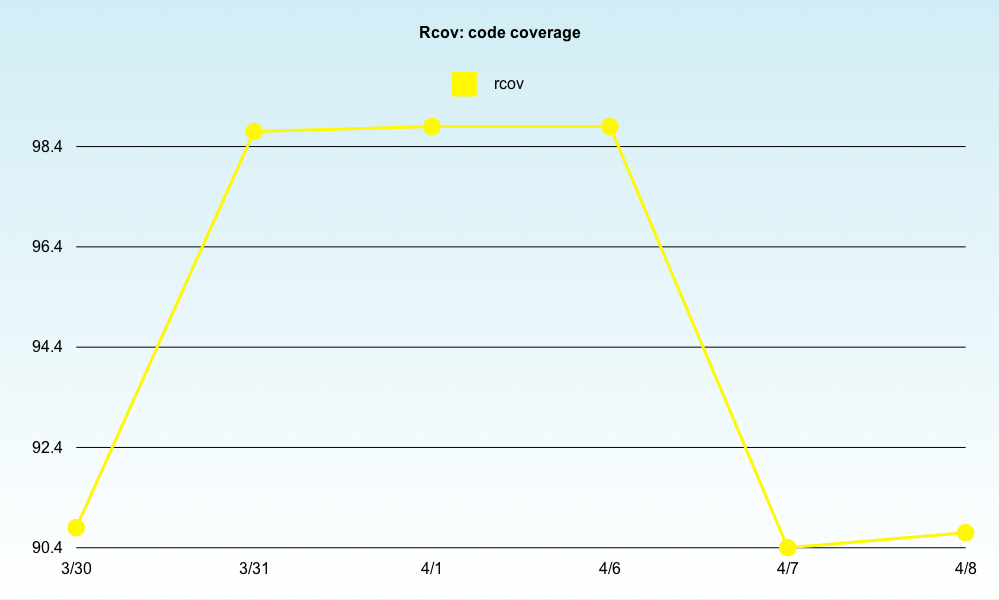
\includegraphics[width=\textwidth]{rcov.png}
	%		\fi
	%	\caption{Test coverage \% reported by Rcov in the main branch over time.}
	%	\label{fig:rcov}
	%\end{figure}
	
	%As of this writing there are 444 Lines of Code in the master branch (trunk) in the repository. These lines are 90.7\% covered by 112 assertions in 91 tests.
	%As can be seen in the diagram over test coverage (available in \figurename{} \ref{fig:rcov} on \pagename{} \pageref{fig:rcov}) the test coverage has decreased during the second week. This is mainly due to a few lines in the server handling remote players  lacks proper tests.
	
	%	\begin{figure}[h!]
	%		\centering
	%			\ifpdf
	%				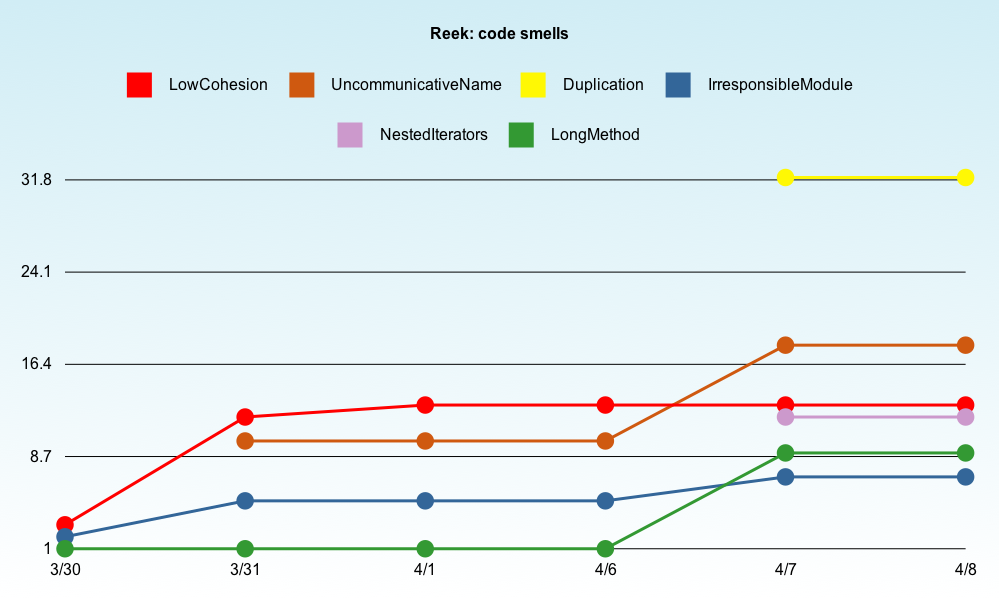
\includegraphics[width=\textwidth]{reek.png}
	%			\fi
	%		\caption{Potential problems detected by Reek}
	%		\label{fig:reek}
	%	\end{figure}
	
	%	There are also a few classes with a possible need for refactorization. A diagram over problems reported by Reek\footnote{Reek, the code smell detector for Ruby. http://wiki.github.com/kevinrutherford/reek/} is available in \figurename{} \ref{fig:reek} on \pagename{} \pageref{fig:reek}.
		
	%	Most of the problems with regards to the server will be removed during refactorization after the functionality of the server is completed. Many of the remaining problems are in the code for the prototype of the GUI which will also be rewritten.
	
	\section{Earned Value}
	\begin{table}[t!]
	\vspace{30mm}	
	\centering
	\begin{tabular}{*{9}{l}}
	    \multicolumn{1}{c}{\begin{rotate}{45}\textbf{Milestone}\end{rotate}} &
		 \multicolumn{1}{c}{\begin{rotate}{45}\textbf{BCW}\end{rotate}} & 
		 \multicolumn{1}{c}{\begin{rotate}{45}\textbf{ACWP}\end{rotate}} &
		 \multicolumn{1}{c}{\begin{rotate}{45}\textbf{Planned Completion Date}\end{rotate}} &
		 \multicolumn{1}{c}{\begin{rotate}{45}\textbf{Actual Completion Date}\end{rotate}}  &
		 \multicolumn{1}{c}{\begin{rotate}{45}\textbf{BCWP (2010-04-09)}\end{rotate}} &
		 \multicolumn{1}{c}{\begin{rotate}{45}\textbf{BCWS (2010-04-09)}\end{rotate}} \\
% TODO: Set new values, not touched since progress report.
\hline
\textbf{Interfaces \& Tests}	 & 06:00	 & 04:30	& 2010-03-30	 & 2010-03-30	& 06:00		& 06:00 \\
\textbf{Computer Players}        & 18:00	 & 06:20	& 2010-04-06	 & 2010-04-07	& 18:00		& 18:00 \\
\textbf{Rules}			 & 06:00	 & 06:20	& 2010-04-07	 & 2010-03-31	& 06:00		& 06:00 \\
\textbf{UI Designed}		 & 10:00	 & 09:05	& 2010-04-07	 & 2010-04-06	& 10:00		& 10:00 \\
\textbf{Server}			 & 20:00	 & -		& 2010-04-08	 & -		& -		& 20:00 \\
\textbf{UI Implemented}		 & 20:00	 & -		& 2010-04-13	 & -		& -		& -	\\
\textbf{Integration}		 & 06:00	 & -		& 2010-04-14	 & -		& -		& -	\\
\hline
\textbf{Project plan}		 & 20:00	 & 20:05	& 2010-03-29	 & 2010-03-29	& 20:00		& 20:00 \\
\textbf{Progress Report}	 & 15:00	 & 26:10	& 2010-04-08	 & 2010-04-08	& 15:00		& 15:00 \\
\textbf{Final Report}            & 25:00	 & -		& 2010-04-15	 & -		& -		& -	\\
\hline
\hline
\textbf{Total}			 & 146:00	 & 72:30	& -		 & -		 & 75:00	& 95:00 \\
\hline
		\hline
	\end{tabular}
	\vspace{5mm}
	\begin{tabular}{*{9}{l}}
	    EV  & = & BCWP/BAW  & = & 75/146  & = & 0.514 & $\Rightarrow$ & 51\% complete as of 2010-04-09 \\
	    SPI & = & BCWP/BCWS & = & 75/95   & = & 0.789 & $\Rightarrow$ & 21\% behind schedule \\
	    CPI & = & BCWP/ACWP & = & 75/72.5  & = & 1.034 & $\Rightarrow$ & Expected total effort = 141h \\
	\end{tabular}{}
	\caption{Table of earned value}
	\label{table:ev}
	\end{table}
	\nomenclature{BCW, Budgeted Cost of Work}{Estimated(planned) effort of the tasks.}
	\nomenclature{ACWP, Actual Cost of Work Performed}{Actual effort of the tasks that have been completed by a specific time.}
	\nomenclature{BCWP, Budgeted Cost of Work Performed}{Estimated effort of the tasks that have been completed by a specific time.}
	\nomenclature{BCWS, Budgeted Cost of Work Scheduled}{Estimated effort of the tasks that were scheduled to be completed by a specific time.}
	\nomenclature{EV, Earned Value}{Amount of work completed completed by a specific time in percent.}
	\nomenclature{SPI, Scheduled Performance index}{Percentage of scheduled work completed by a specific time.}
	\nomenclature{CPI, Cost Performance Index}{A value indicating time spent vs. time scheduled. Value under 1 indicates more time was spent than scheduled.}
	\vspace{2mm}

	
	\section{Individual Effort}

	% TODO: Update values!
	\begin{table}
		\centering
	\begin{tabular}{l ccc}
		\textbf{Milestone}		
							& \textbf{Emil} & \textbf{Fredrik}	& \textbf{Marcus} \\
		\hline
		\textbf{Interfaces \& Blackbox tests}	& 02:15		& -			& 02:15 \\
		\textbf{Computer Players}		& 03:10		& 01:00			& 02:10 \\
		\textbf{Rules}				& 07:30		& -			& - \\
		\textbf{UI Design}			& 00:20		& 00:20			& 08:25 \\
		\textbf{Server}				& 12:15		& -			& 03:10 \\
		\textbf{UI Implemented}			& -		& -			& 10:54 \\
		\hline   
		\textbf{Project plan}			& 07:35		& 05:00			& 07:30 \\
		\textbf{Progress Report}		& 10:55		& 11:43			& 03:30 \\
		\hline
		\textbf{Other (Metrics, Tracking etc.)} & 01:30		& 04:00			& - \\
		\hline
		\hline
		\textbf{Total}				& 45:30		& 22:03			& 38:24 \\
		\hline
		\hline
	\end{tabular}
		\caption{A table of the individual effort spent by the team members}
		\label{tab:effort}
	\end{table}

	A table over the individual effort is avaliable in \tablename{} \ref{tab:effort} on \pagename{} \pageref{tab:effort}. Right now there is a quite large difference between time spent by the different team members.

	\section{Problems Encountered}
	One of the problems we have had was related to Ruby/Tk. Although a relatively competent framework for creating graphical user interfaces we ran into a few problems when combining it with Distributed Ruby. The biggest issue so far has been related to updating the user interface on callbacks from the server.
	
	Apart from a few smaller glitches we had initially with Distributed Ruby the biggest problem we have had so far was related to updating the user interface when a call came from the server. The user interface elements wouldn't update even if the associated TkVariable did.

	Another problem was caused by our choice of language. Almost all time spent on programming for Fredrik has gone into learning Ruby and understanding the code written by the other team members. That has forced the other members to be the main programmers in this project.
	
	\section{Conclusions}

\clearpage
\appendix
\printglossary
	
\end{document}
